The proposed algorithm to identify characters in real time is a dynamic time warping similarity search. 

\marginpar{
\vspace{-2in}
\begin{figure}
  \begin{center}
  \subfigure[Euclidean distance]{
    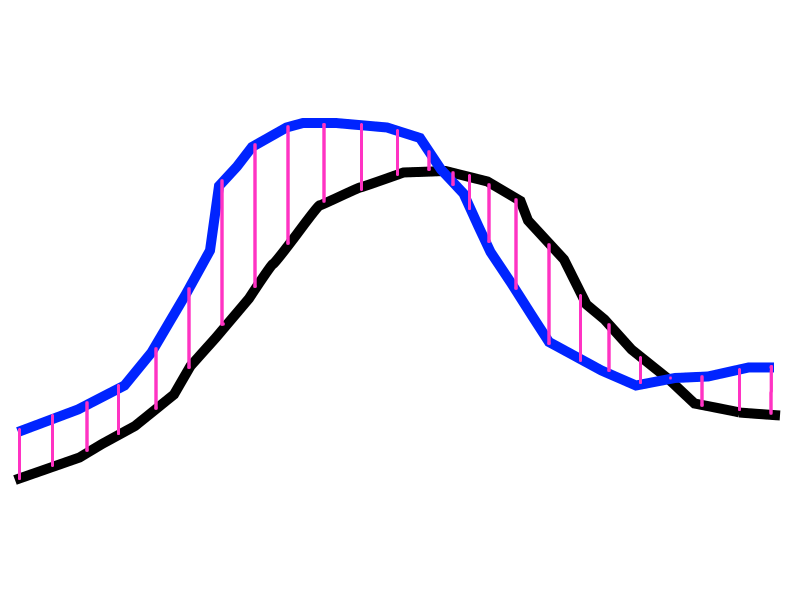
\includegraphics[width=1.8in]{images/dtw-raw.PNG}
  }
  \subfigure[Warping distance]{
    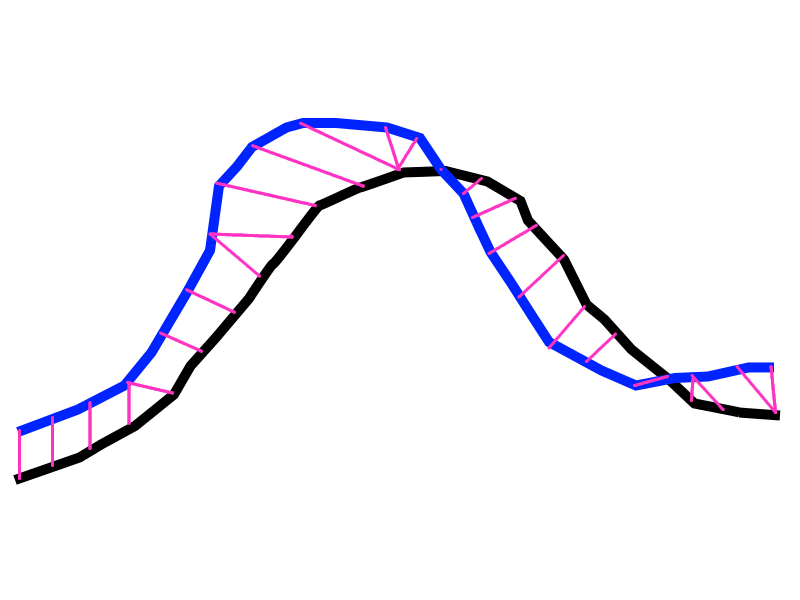
\includegraphics[width=1.8in]{images/dtw-window.PNG}
  }
  \caption{Similarity measures}
  \label{fig:teaser}
  \end{center}  
\end{figure}
}

The input is a data time series, \(D\), and a collection of candidate time series, \( C = \{c_1, c_2, c_3, ..., c_n\}\).
Each time series is multivariate as each element of the time series is a 3D point, \(\{x_i, y_i,z_i\}\)
The first goal is to have some sort of similarity search algorithm.
\begin{algorithm}[h]
 \SetKwData{Best}{best}
 \SetKwData{Location}{location}
 \SetKwData{Distance}{distance}
 \SetKwData{Loc}{loc}
 \SetKwData{D}{D}
 \SetKwData{C}{c}
 \SetKwData{Collection}{C}

 \SetKwFunction{Search}{Search}

 \SetKwInOut{Input}{input}\SetKwInOut{Output}{output}

 \Input{\Collection, \D}
 \Output{Matches of all the candidates to \D}
 Distances$\leftarrow$Map();\\
 \For{\C in \Collection}{
    \Distance, \Location$\leftarrow$\Search{\C, \D}\;
    Distances[\C]$\leftarrow$(\Distance,\Location);
 }
 \Return{Distances}
 \caption{High level database search algorithm}
\end{algorithm}

The similarity search will consist of a sweep across the data time series, checking every subsequence against the candidate and returning the best match.
Both the candidate and all subsequences are z-normalized in the process.
\begin{algorithm}[h]
 \SetKwData{Best}{best}
 \SetKwData{Location}{location}
 \SetKwData{Distance}{distance}
 \SetKwData{Loc}{loc}
 \SetKwData{D}{D}


 \SetKwFunction{Similarity}{Similarity}

 \SetKwInOut{Input}{input}\SetKwInOut{Output}{output}

 \Input{c, D}
 \Output{distance, location}
 \Best$\leftarrow -\infty$\;
 \For{\Loc in \D}{
    \Distance$\leftarrow$\Similarity{c,\D}\;
    \If{\Distance $<$ \Best}{
        \Location$\leftarrow$ \Loc\;
        \Best$\leftarrow$\Distance\;
    }
 }
 \Return{distance, location}
 \caption{Similarity search algorithm}
\end{algorithm}

The dynamic time warping algorithm is used as a similarity metric between vectors. It is a generalization of the Euclidean distance metric but chooses the closest point within a certain time window, rather than creating a one-to-one mapping of points. When the time window is 0, DTW reduces to Euclidean distance.

